\chapter{Surrogate based shape optimization}
\label{optimization}
The process employed for aerodynamic shape design can be a direct or indirect shape optimization. In direct shape optimization approach, the process starts with random combinations of design parameters. An optimization algorithm is used which requires CFD simulation at each iteration to find parameters in the design space for minimum drag. This approach requires large number of CFD simulations and takes significant amount of time to complete the optimization process. Also, grid influences the solution considerably. So, using this method we can no longer guarantee that the changes in the solution of objective function value is because of the changes in the parameters of CAD or if they are coming from changes in the grid. Solution for above problem can be answered by developing a surrogate model.
\begin{figure}[H]
	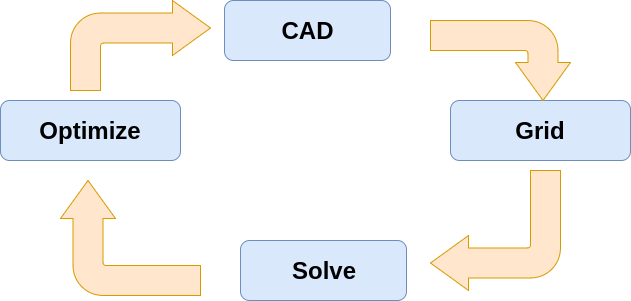
\includegraphics[width=\textwidth]{optimization/closed_loop.png}
	\caption{Direct shape optimisation approach}
	\label{Closed Optimization loop} %      only if needed
\end{figure}

\section{Surrogate model}

 Surrogate model is one of the mathematical and statistical techniques used to develop adequate functional relationship between an objective function y(x) and the control or design variables $ x_1 , x_2 .... x_k $. In our case, The model acts like a black box for aerodynamic parameters. Given the set of design variables, the model should give volumetric drag coefficient as shown in Fig. \ref{Surrogate model} . The work flow associated with the development of a surrogate model is shown in Fig. ~\ref{fig:work flow for the development of a surrogate model} . To develop an accurate surrogate, we need to carry out large number of CFD simulations. Creating geometry every time and meshing them is possible but takes a lot of time. Instead we can automate all the processes right from geometry creation to meshing and solving. This has become possible with OpenFOAM\textsuperscript{\textregistered}.

\begin{figure}[H]
	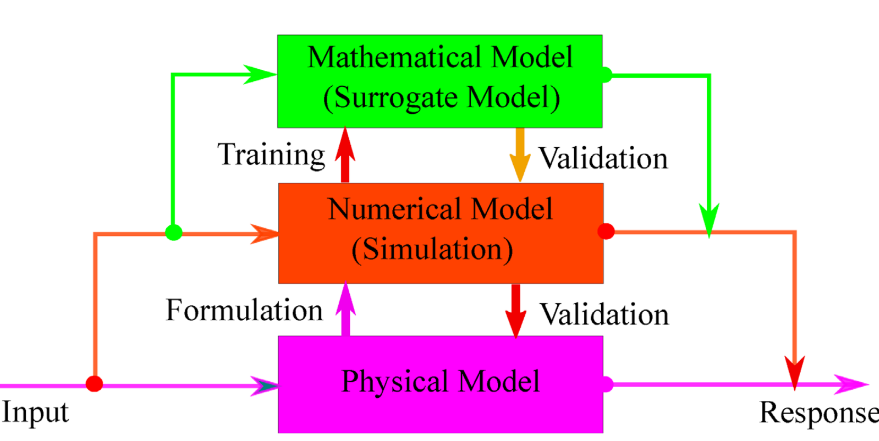
\includegraphics[width=\textwidth]{optimization/surrogate.png}
	\label{Surrogate model} %      only if needed
	\caption{Surrogate model definition [\citenum{alam2017thesis}]}
\end{figure}

%\begin{figure}[htbp]
%	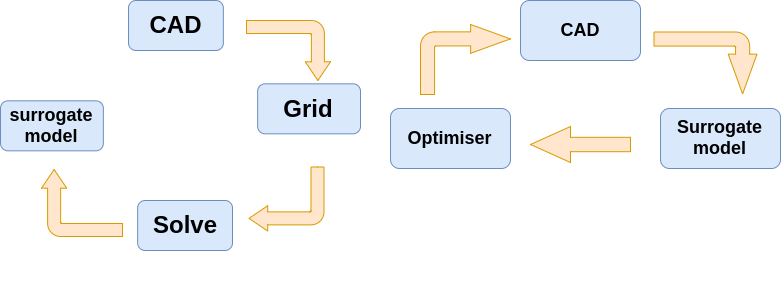
\includegraphics[width=\textwidth]{optimization/model.png}
%	\caption{Broken Optimization loop with the use of surrogate model}
%	\label{Broken Optimization loop with the use of surrogate model} %      only if needed 
%\end{figure}

\begin{figure}[htbp]
	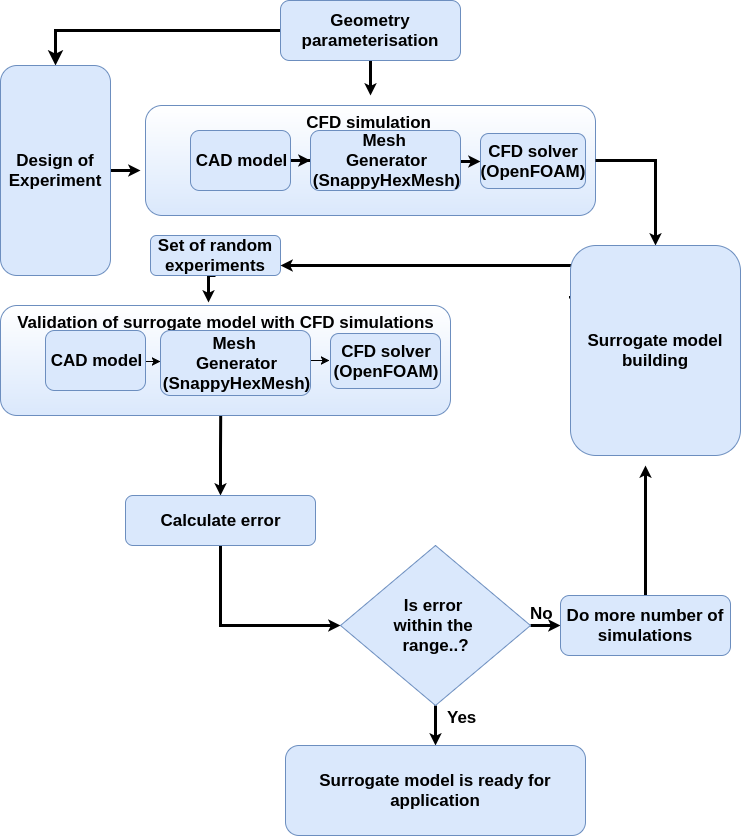
\includegraphics[width=\textwidth]{optimization/flow_chart.png}
  
	\caption{Work flow for the development of a surrogate model [\citenum{OsamaAbdulGhani2013}]}
	\label{fig:work flow for the development of a surrogate model} %      only if needed
\end{figure}


\section{Design of Experiments}
\label{DOE}
Design of Experiments is a technique used to extract maximum possible information from minimum number of computational experiments. This can be accomplished by the selection of a proper and robust scheme for DOE (Design of Experiments). In the present study, an open-source software named Surrogates Toolbox Version 3.0 (Viana, 2011) was used. Apart from many other important features, the toolbox provides an access to several varieties of widely used DOE models. Of the many DOE models available in the toolbox, Optimal Latin Hypercube Sampling (OLHS) generated using translational propagation algorithm (TPA) Viana[\citenum{Viana2011}] was chosen, mainly due to its orthogonal structure. Fig. \ref{OLHS Sampling} shows sampling distribution of points in a unit square.

\begin{figure}[htbp]
	\centering
	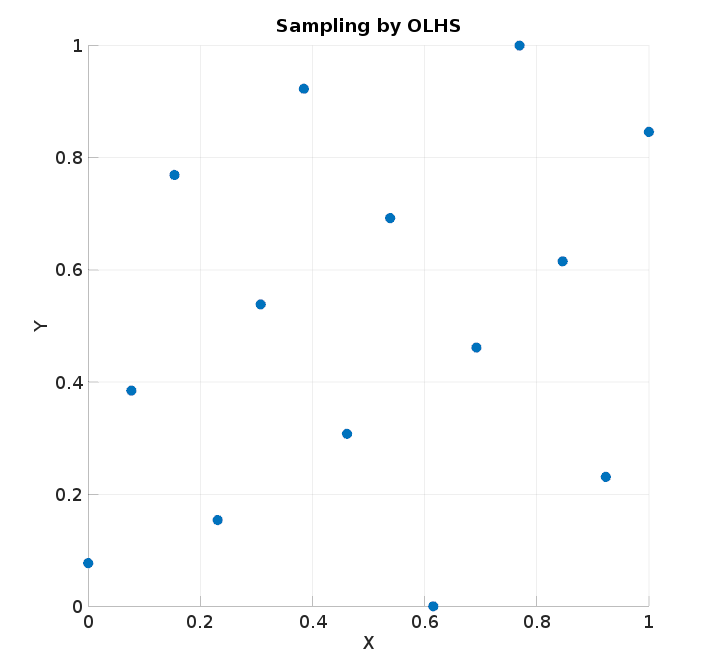
\includegraphics[width=200 pt]{optimization/OLHS_DOE}
	\caption{Sampling of unit square using OLHS }
	\label{OLHS Sampling}
\end{figure}

 The number of design experiments depends on the number of shape parameters used for defining geometry. A rule of thumb is that the number of design experiments should be ten times the number of shape parameters. However the actual number is decided by obtaining error between surrogate model results and actual CFD results. For the surrogate model to be acceptable, the error should be less than 2 percent. Alam \citenum{alam2016mdo} reported to have made 60 design experiments while developing his surrogate model for 2D bodies of revolution shapes. Kale et al. [\citenum{Kale2005a}] reported to have studied about 600 feasible shapes using ANSYS\textsuperscript{\textregistered} \textit{Fluent} CFD package while developing quadratic response surface using Design Expert package.

For numerical experiments, Kriging surrogate model is reported to be best \citenum{viana2014metamodeling}. Kriging is named after the pioneering work of the South African mining engineer D. G. Krige. It is an interpolating method modeled by a Gaussian process governed by prior co-variances, which features the observed data at all design points. Kriging provides a statistic prediction of an unknown function by minimizing its Mean Squared Error (MSE).

The Kriging method in its basic formulation estimates the value of a function at some un sampled location as the sum of two components: the linear regression model $ f_i (x) $ (e.g., polynomial trend) of the data with p regressors modeling the drift of the process mean, i.e., the trend, over the domain, and a systematic departure representing low (large scale) and high frequency (small scale) variation components, respectively.

\section{Building the surrogate model}
A brief overview of different surrogate models by Luo et al.[\citenum{luo2014comparison}] is given below.
\subsection{Polynomial response surface}
Polynomial response surface is the simplest approximation method to build surrogate models Forrester et al.[\citenum{forrester2009recent}]. The most widely used polynomial response surface model is the second-order polynomial model which has the following form.
\begin{equation}
y = \beta _{0} + \sum_{i=1}^{n} \beta _{i} x_{i} + \sum_{i=1}^{n} \sum_{j \ge i}^{n} \beta _{ij} x_{i} x_{j} + ..
\end{equation}

where $ \beta _{0},\ \beta_{i},\ \beta _{ii},$ and $ \beta _{ij} $ are the regression coefficients, n is the number of variables, xi and xj are the variables. Using least square method (LSM), the regression coefficients can be solved.

\subsection{Radial Basis Function}
RBF is a 3-layer feed forward neural network consisting of an input layer, a hidden layer, and an output layer Shen et al.[\citenum{shen2011forecasting}]. X is an N dimensional input vector. The output of the neurons in the RBF hidden layer is assumed as:

\begin{equation}
q_{i} = \varPhi(|| X - c_{i} ||)
\end{equation}

where $ c_{i} $ is the center associated with the ith neuron in the radial basis function hidden layer, i = 1, 2,...,H, where H is the number of hidden units, $ || X - c_{i} || $ is the norm of $ X − c_{i} $, $ \varPhi (.) $ is a radial basis function [\citenum{chen1991orthogonal}]. Outputs of the kth neuron in RBF output layer are linear combinations of the hidden layer neuron outputs as:

\begin{equation}
y_{k} = \sum_{i=1}^{H} w_{ki} q_{i} - \theta _{k} \quad (k = 1, 2,...,M)
\end{equation}
where $ w_{ki} $ is the connecting weights from the $ i^{th} $ hidden layer neuron to the $ k^{th} $ output layer, $ \theta _{k} $ is the threshold value of the $ k^{th} $ output layer neuron.

\subsection{Kriging}
The kriging method was developed by the French mathematician Georges Matheron based on the Master$ ' $s thesis of Daniel Gerhardus Krige [\citenum{matheron1963principles}], it was first used as a geo statistical method. Sacks et al.[\citenum{sacks1989design}] firstly introduced Kriging method as a surrogate modeling method, in the paper of Sacks et al.[\citenum{sacks1989design}], Kriging surrogate model was also called design and analysis of computer experiment (DACE). The \textit{Kriging} model is a combination of two components [\citenum{queipo2005surrogate}]: deterministic functions and localized deviations.

\begin{equation}
Y(x) = \sum_{i=1}^{k} f_{i} (x) \beta _{i} + z(x)
\end{equation}

where $ \sum_{i=1}^{k} f_{i} (x) \beta _{i} $ is the term of deterministic functions, $ \beta$ are coefficients of deterministic functions, fi(x) are k known regression functions, which are usually polynomial functions. z(x) is term of localized deviations with mean zero, variance $ \sigma ^2$, and covariance expressed as:

\begin{equation}
Cov[z(x_{i}),z(x_{j})] = \sigma ^{2} R (x_{i},x_{j})
\end{equation}

where $ R (x_{i},x_{j}) $  is the correlation function between any two of the ns samples The common types of correlation functions are linear function, exponential function, Gauss function, spline function, etc. (Ryu et al. 2002). The prediction of un sampled points response y(x) can be expressed as:

\begin{equation}
\hat{y}(x) = f(x)^{T} \beta + r^{T} R^{-1} (Y - F \beta )
\end{equation}

where Y is the vector of ns samples response, r is the correlation vector between samples and prediction points.


\begin{eqnarray}
& r = [R(x,x_{1}),R(x,x_{1}),....,R(x,x_{1}) ]^{T} \\
& F = [f(x_{1}), f(x_{2}),.....f(x_{n_{x}}) ]^{T} .
\end{eqnarray}

\section{Toolbox used for different surrogate models}

Table \ref{Different surrogates used during this investigation} details the different surrogates used during this investigation. The SURROGATES toolbox was also used for easy manipulation of the surrogates.

Table \ref{Different surrogates used during this investigation}: Setup for the set of used surrogates. The  DACE [\citenum{lophaven2002dace}], RBF[\citenum{Jekabsons2009}] and SURROGATES [\citenum{Viana2011}] toolboxes were used to run the kriging, radial basis function and polynomial response surface respectively.

\begin{table}[H]
	\centering
	\caption{Different surrogates used during this investigation}
	\label{Different surrogates used during this investigation}
	%\begin{ruledtabular}
	\begin{tabular}{ll}
		\hline \hline
		Surrogate & Details    \\ \hline \hline
		KRG	 & Kriging model: constant trend function and Gaussian correlation \\
		PRS & Polynomial response surface: Second degree polynomial \\
		RBF  & Radial basis function: Multiquadric basis function \\
		\hline \hline
	\end{tabular}
	%	\end{ruledtabular}
\end{table}


\section{Test Function for Kriging Surrogate Model}
\label{test function}
The Himmelblau function is taken as a test function.  It has one local maxima and four local minima in the domain x = [-6,6] and y = [-6,6]. The function is defined as 
\begin{equation}
f(x,y) = (x^2 + y - 11)^2  + (x + y^2 - 7)^2 
\end{equation}
\begin{equation}
x \in [-6,6] ;\quad y \in [-6,6]
\end{equation}

It has one local maximum at x=-0.270845 and y=-0.923039 where f(x,y)=181.617, and four identical local minima:
\begin{align}
&f( 3.0000 , 2.0000 )=0.0 \\
&f( -2.8051 , 3.1313 )=0.0 \\
&f( -3.7793 , -3.2831 )=0.0 \\
&f( 3.5844 , -1.8481 )=0.0 \\
\end{align}

If a small number of design points are used to create a surrogate model, then the approximate model created is prone to large errors at the trial points. However, the prediction accuracy of a surrogate model cannot be improved merely by taking larger number of design points; that is a function of its behaviour, design space and the required accuracy. Fig. \ref{fig:Root Mean Square Error with Design Points considered} shows the effect of increase in number of design points on the Root Mean Square Error (RMSE) of this test function. It is seen that the prediction accuracy of the model improves till 120 design points, after which addition of more design points does not approximate model for surrogate on the right with all the design points and test points. The actual value fo the function and predicted value from the surrogate model at test points are seen to match with each other within 1\%.

\begin{figure}[H]
	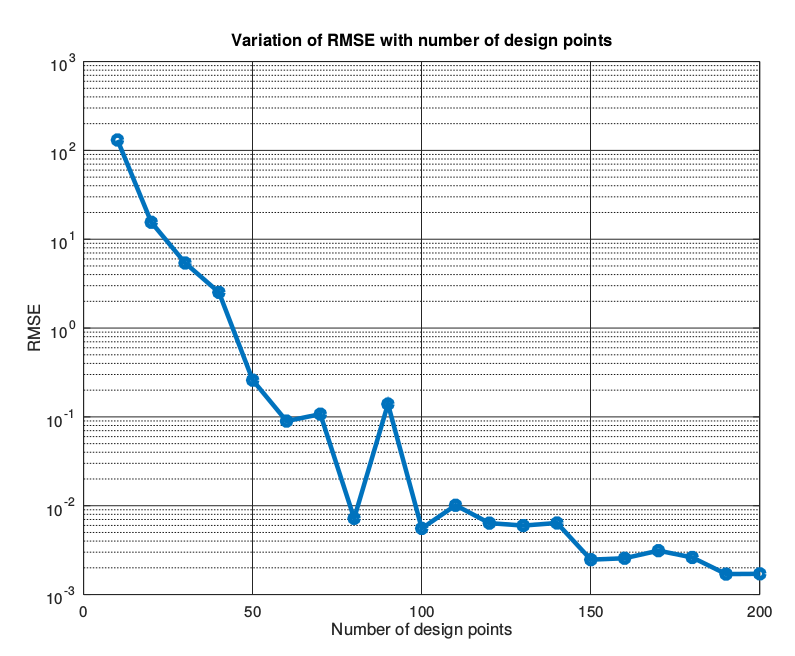
\includegraphics[width=\textwidth]{optimization/RMSE_analysis.png}
	\caption{Root Mean Square Error with Design Points considered}
	\label{fig:Root Mean Square Error with Design Points considered} %      only if needed
\end{figure}


\begin{figure}[H]
	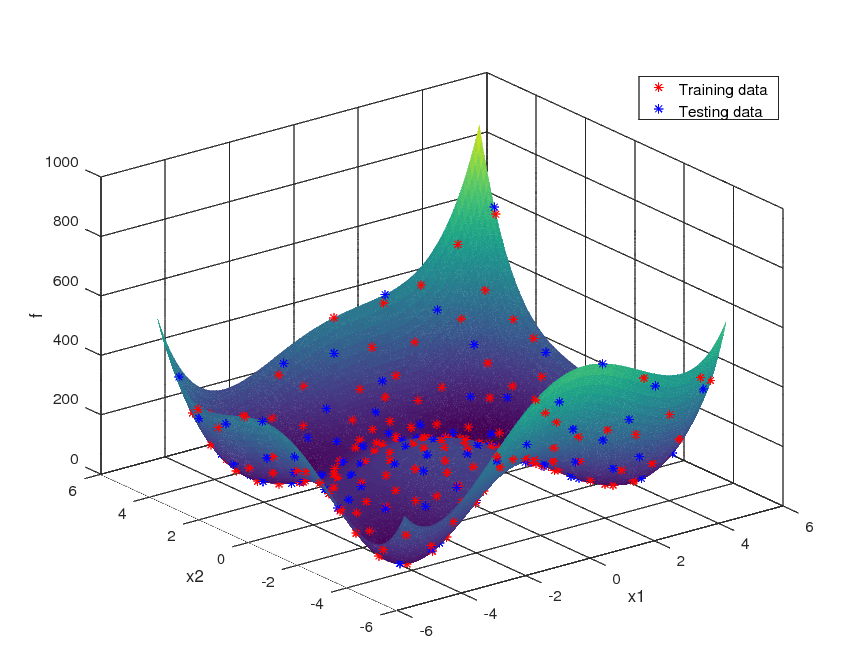
\includegraphics[width=\textwidth]{optimization/Himmel_blau_fcn.png}
	\caption{Comparison of Himmelblau function with its Surrogate Model}
	\label{fig:Comparison of Himmelblau function with its Surrogate Model} %      only if needed
\end{figure}

\section{Coupling of Genetic Algorithm, Surrogate model and testing for modified Himmelblau functions}
\label{Modified Himmelblau function}
It is a well known fact that evolutionary algorithms like Genetic algorithm searches for global minimum and outputs that global minimum as final answer. Unlike gradient based methods, it should not get struck in local minimum. In order to check this, we modify the existing Himmelblau function. This is because actual Himmelblau function has four identical local minimum and don't have any global mimima. So, we modify it by adding the term $  0.01* (x + 3.7793)^2 + (y + 3.2832)^2 $. This term is added to the function value evaluated at all points except (-3.7793,-3.2832). Hence we obtained modified Himmelblau function with one global minima at (-3.7793,-3.2832) and three local minima at other three points. If we optimise this modified Himmelblau function using Genetic algorithm, we have to get the final answer as (-3.7793,-3.2832). The same answer is expected using surrogate model for the modified Himmelblau function. The obtained results are shown in Table \ref{Results obtained for modified Himmelblau function}

The genetic algorithm code used is a MATLAB code is written by Xavier [\citenum{Xavier}]. The input parameters used are default values given by author and are specified in Table \ref{Genetic algorithm parametres}. NVAR is the number of variables (2 for present case).
\begin{table}[H]
	\centering
	\caption{Genetic algorithm parameters}
	\label{Genetic algorithm parametres}
	%\begin{ruledtabular}
	\begin{tabular}{ll}
		\hline \hline
		Parameter & Value \\
		\hline
		Population size & NVAR*50 \\
 		Crossover probability & 0.9 \\
 		Mutation probability & 0.1 \\
 		Number of generation & NVAR*20+10 \\
 		Selection scheme & Roulette wheel selection method \\
		
		\hline \hline
		
	\end{tabular}
	%	\end{ruledtabular}
\end{table}


\begin{table}[H]
	\centering
	\caption{Results obtained for modified Himmelblau function}
	\label{Results obtained for modified Himmelblau function}
	%\begin{ruledtabular}
	\begin{tabular}{llll}
		\hline \hline
		& X & Y & Function value \\ \hline
		Actual Function & -3.7793 &-3.2832 &1.6725e-11 \\
		Surrogate model & -3.7791 &-3.2828 & 2.5643e-03 \\ \hline
		\% error & 0.006 & 0.013 & NA \\
		\hline \hline
		
	\end{tabular}
	%	\end{ruledtabular}
\end{table}

To explain the query of what happends if we take less number of design points while fitting the surrogate model, consider modified Himmelblau function discussed in Section \ref{Modified Himmelblau function}. From Fig. \ref{fig:Root Mean Square Error with Design Points considered}, we can infer that we need at least 150 design points to get develop a surrogate model which mimics actual Himmelblau function. But instead of 150 points, lets take only 20 points and construct a Kriging surrogate model and find the optimal point. It is already known that the optimal points is  (-3.7793,-3.2872). If we couple the genetic algorithm optimizer with surrogate model developed using only 20 points, we get the following results.
\begin{table}[H]
	\centering
	\caption{Results obtained for 20 design points}
	\label{Results obtained for 20 design points}
	%\begin{ruledtabular}
	\begin{tabular}{llll}
		\hline \hline
		& X & Y & Function value \\ \hline
		Actual Function & -3.7793 &-3.2832 &1.3278e-13 \\
		Surrogate model & -3.2205 &-2.9549 & -6.3131 \\ \hline
		\% error & 14.79 & 10.00 & NA \\
		\hline \hline
	\end{tabular}
	%	\end{ruledtabular}
\end{table}
From the above table we may see that if the number of design points used to train the model are low and if this model is coupled with optimizer, we end up getting sub-optimal solution with some percentage error.





%%


%%% Local Variables: 
%%% mode: latex
%%% TeX-master: "../mainrep"
%%% End: 
